\section{Problem Definition}

\subsection{Markov Decision Process and Agent-Environment Interface}
A RL problem is usually represented as a \textbf{Markov Decision Process (MDP)}.
MDP is four-tuple $(\mathcal{S}, \mathcal{A}, R, P)$:
$\mathcal{S}$ is a set of states that forms the \textbf{state space}
$\mathcal{A}$, is a set of actions that forms the \textbf{action space};
$P(s, a, s') = Pr[ S_{t+1} = s' \mid  S_t = s, A_t = a]$ is the \textbf{transition probability function};
$R(s, a, s')$ is the \textbf{reward function}.
We use the \textbf{agent-environment interface} to solve a problem formulated as an MDP.
Figure \ref{fig:agent_environment_interface} illustrates the agent-environment interface.
The MDP is represented as the \textbf{environment}.
The decision maker that interacts with the environment is called the \textbf{agent}.
At each time step $t$, the agent starts at state $S_t \in \mathcal{S}$, takes an action $A_t \in \mathcal{A}$,
transitions to state $S_{t+1} \in \mathcal{S}$ based on the transition probability function $P(S_{t+1} \mid S_t, A_t)$,
and receives a reward $R(S_t, A_t, S_{t+1})$.
These interactions yield a sequence of actions, states, and rewards $S_{0}, A_{0}, R_{1}, S_{1}, A_{1}, R_{2}, \dots$.
We call this sequence a \textbf{trajectory}.
When a trajectory ends at a terminal state $S_T$ at time $t = T$, this sequence is completed and we called it an \textbf{episode}.

\begin{figure}[ht]
    \centering
    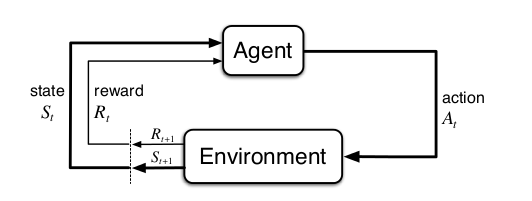
\includegraphics[scale=0.5]{assets/agent_environment_interface.png}
    \caption[]{Agent-Environment Interface}
    \label{fig:agent_environment_interface}
\end{figure}
\note{my notation is messed up but I will fix them later for sure.}

At each state $s$, then agent takes an action based on its \textbf{policy} $\pi(a \mid s)$.
This policy represents the conditional probability of the agent taking an action given a state so that
$\pi(a \mid s) = Pr[ A_{t} = a \mid  S_t = s]$.
One way to specify the goal of the agent is to obtain a policy that maximizes the sum of expected reward from any state $s$
\begin{align}
    \label{eq:maximize_reward_undiscounted}
    \mathit{E}_{\pi}\left[\sum_{k=0}^{T}  R_{t+k+1} \mid S_t = s\right]
\end{align}
where $\mathit{E}_{\pi}$ denotes the expectation of the agent following policy $\pi$.
Another way is to also use a discount factor $\gamma$ so to favor short-term rewards
\begin{align}
    \label{eq:maximize_reward_discounted}
    \mathit{E}_{\pi}\left[\sum_{k=0}^{T} \gamma^{t} R_{t+k+1} \mid S_t = s\right]
\end{align}
Notice that (\ref{eq:maximize_reward_undiscounted}) is a special case of (\ref{eq:maximize_reward_discounted}) where $\gamma = 1$.
\note{Maybe I should use one formula here to unify both.}

% \note{also describes policy $\pi$}
% \note{address this is the most common formulation and how different libraries implement the interface}

% \subsection{Shortcomings of the Agent-Environment Interface for General Game Playing}
% % \note{I'm not sure if I should address these separatly.}
% \subsection{Multi-Agent Games}
% \note{address OpenSpiel's design multiple agents}
% \subsection{Partial Observability}
% \note{address POMDP}
% \subsection{Environment Stochasticity}
% \note{address OpenSpiel's design of random node}
% \subsection{Episodic vs Continuous}
% \note{barely seen in the literature, need more literature review}
% \subsection{Self-Observability}
% % \note{agent needs to be able to observe itself}
% \subsection{Environment Output Structure}
% % The agent-environment interface specifies two return types from the environment, namely the \textbf{observation} and the \textbf{reward}.
% % All environment implementations used in the RL field follow 